\bibliographystyle{babplain-fl}

\chapter{Ejemplos de análisis amortizado}
\label{cha:ejemplos-amortizado}

  Trataremos en detalle algunos ejemplos adicionales
  de análisis amortizado para estructuras simples,
  de aplicación práctica.
  Parte de lo siguiente se adapta de Fiebrink~%
    \cite{fiebrink07:_amortized_analysis_explained}.

\section{Listas autoorganizantes}
\label{sec:list-autoorganizantes}

  Este es un ejemplo interesante
  en que el análisis compara respeto del algoritmo óptimo.
  El modelo no es demasiado realista,
  Es parte de la discusión de Tarjan~%
    \cite{sleator85:_amort_effic_list_updat_pagin_rules},
  quien resume resultados previos
  y discute varias otras situaciones afines,
  de aplicación directa.

  El modelo es de una lista,
  que se accede secuencialmente.
  En muchas aplicaciones,
  las referencias tienen localidad,
  un objeto accedido al instante \(t\)
  es más probable de ser accedido nuevamente poco después de \(t\).
  Para favorecer accesos futuros,
  el elemento buscado se mueve al principio de la lista
  (esta heurística se llama \emph{\foreignlanguage{english}{Move To Front}},
   abreviado MTF).

  Acceder al objeto en la posición \(i\) tiene costo \(i\),
  y un par de objetos vecinos pueden intercambiarse en tiempo constante.
  Con esto,
  el acceder al objeto en posición \(i\) tiene costo \(2 i - 1\)
  (\(i\) para hallarlo,
   luego \(i - 1\) intercambios para llevarlo al comienzo).

  Usamos análisis amortizado para demostrar que el rendimiento de MTF
  siempre está dentro de un factor de \num{4} de \emph{cualquier} algoritmo,
  incluso del óptimo,
  sin suposiciones sobre localidad de referencia.
  Sea \(A\) una lista ordenada,
  en que los elementos mantienen posiciones fijas,
  definimos el potencial de MTF al instante \(t\)
  como dos veces el número de objetos cuyo orden en la lista de MTF
  difiere del orden de la lista \(A\)
  (el número de inversiones).
  Por ejemplo,
  si la lista de \(A\) es \(\langle a, b, c, d, e \rangle\)
  y la de MTF es \(\langle a, d, b, c, e \rangle\),
  \(\Phi = 2 \cdot 2 = 4\)
  por \(b\) y \(c\) respecto de \(d\).
  Claramente,
  el potencial nunca es negativo,
  y a \(t = 0\) es cero,
  ambos comienzan con la misma secuencia.
  El costo amortizado es una cota superior
  al costo de una secuencia de operaciones.

  Considere el acceder al objeto \(x\),
  que está en la posición \(k\) de la lista de MTF
  y en la posición \(i\) en la de A.
  El costo en MTF es \(2 k - 1\),
  el costo en A es \(i\).
  Mover \(x\) al comienzo invierte el orden de los \(k - 1\) pares
  de elementos en posiciones \num{1} a \(k - 1\) con \(x\),
  todos los demás pares se mantienen.
  En la lista de A hay \(i - 1\) objetos antes de \(x\),
  todos ellos terminan después de \(x\) luego de promover a \(x\) en MTF.
  Se añaden a lo más \(\min \{ k - 1, i - 1 \}\) inversiones entre las listas.
  Las demás reorganizaciones
  (a lo menos \(k - 1 - \min \{ k - 1, i - 1 \}\))
  resultan en eliminar inversiones
  (las posiciones ahora concuerdan entre A y MTF).
  En consecuencia,
  el cambio de potencial en este acceso está acotado por arriba por:
  \begin{equation*}
    2 ( \min \{ k - 1, i - 1 \} - (k - 1 - \min \{ k - 1, i - 1 \}) )
      = 4 \min \{ k - 1, i - 1 \} - 2 (k - 1)
  \end{equation*}
  En consecuencia,
  el costo amortizado de esta operación es:
  \begin{align*}
    a
      &=   c + \Delta \Phi \\
      &\le 2 k - 1 + 4 \min \{ k - 1, i - 1 \} - 2 (k - 1) \\
      &\le 4 \min \{ k - 1, i - 1 \} \\
      & \le 4 i
  \end{align*}
  O sea,
  el costo de acceso amortizado de MTF está acotado por \num{4} veces el de A.

  Pero lo anterior no considera reorganizaciones que hace A.
  Sea que A intercambia dos objetos.
  Esto no introduce costo adicional para MTF,
  pero el potencial aumenta o disminuye en \num{2}
  (dos objetos cambian de posición),
  y aumenta el costo de acceso en A en \num{1}.
  La cota se mantiene,
  el costo amortizado aumenta a lo más en 2
  y la cota aumenta en \num{4}.
  Esto vale independiente del número de intercambios que hace A.

\section{Splay trees}
\label{sec:splay-trees}

  Supondremos que la terminología sobre árboles binarios de búsqueda
  junto con los algoritmos relevantes de búsqueda, inserción y eliminación
  son conocidos.
  Si no es así,
  revise sus apuntes de estructuras de datos.

  Recuerde que la \emph{profundidad} de un nodo en un árbol binario
  es su distancia a la raíz,
  y su \emph{altura} es la distancia a su hoja descendiente más lejana.
  La altura del árbol es simplemente la altura de su raíz.
  Llamaremos \emph{tamaño} de un nodo al número de nodos en su subárbol.
  El tamaño del árbol es el tamaño de su raíz.

  Un árbol de altura \(h\) tiene a lo más \(2^h\) hojas
  (un simple ejercicio de inducción),
  por lo que un árbol con \(n\) hojas
  tiene altura al menos \(\lceil \log_2 n \rceil\).
  En el peor caso,
  el tiempo para una búsqueda, inserción o eliminación
  es proporcional a la altura del árbol,
  por lo que nos interesa minimizar la altura.
  Lo mejor que podemos hacer
  es mantener \emph{árboles perfectamente balanceados},
  en los cuales cada subárbol
  (recursivamente)
  tiene lo más exactamente posible la mitad de los nodos.
  Esto asegura que la altura sea exactamente \(\lceil \log_2 n \rceil\)
  (otro ejercicio simple de inducción),
  con lo que el peor caso del tiempo de búsqueda es \(O(\log n)\).
  Sin embargo,
  si partimos con un árbol perfectamente balanceado
  una secuencia maliciosa de inserciones y eliminaciones
  puede hacerlo arbitrariamente desbalanceado,
  llevando los tiempos de búsqueda a \(\Theta(n)\).
  Para evitar esto,
  debemos modificar el árbol periódicamente para mantener el balance
  (al menos aproximadamente).
  Hay varios métodos para hacer esto,
  que llevan a árboles binarios con nombres diversos:
  árboles AVL,
  árboles rojo-negro,
  árboles balanceados en altura
  o en peso,
  y otros más.
  Plavec, Vranesic y Brown~%
    \cite{plavec07:_digital_search_trees}
  resumen evaluación experimental de estas
  y otras alternativas.
  El problema de todas ellas es que almacenan información adicional
  necesaria para mantener el balance
  (pueden reusarse bits en desuso para ello,
   pero eso lo hace poco portable),
  y operaciones engorrosas de programar.

  Una alternativa simple,
  que no requiere espacio adicional,
  relativamente simple de programar
  y con tiempo de ejecución amortizado \(O(\log n)\) para todas las operaciones
  son los \emph{\foreignlanguage{english}{splay trees}}
  propuestos por Sleator y Tarjan~%
    \cite{sleator85:_splay_trees}.
  La idea básica es promover a la raíz al nodo resultado de una búsqueda,
  reorganizando el árbol en el proceso.
  Resulta un árbol agradablemente balanceado,
  y en el caso común en que los accesos se aglomeran,
  los elementos buscados frecuentemente estarán cerca de la raíz.
  Eso sí que tienen la desventaja que incluso operaciones de \textquote{solo lectura}
  (búsquedas)
  reorganizan el árbol,
  lo que hace que esta estructura
  lamentablemente no pueda usarse en forma concurrente.

\section{Pairing Heaps}
\label{sec:pairing-heaps}

  En algunas aplicaciones de colas de prioridad
  es importante la operación de modificar la prioridad de un elemento
  (particularmente en algoritmos que trabajan sobre grafos,
   por ejemplo,
   el algoritmo de Dijkstra).
  Esta operación es provista en forma eficiente en el Fibonacci heap,
  de Fredman y Tarjan~%
    \cite{fredman87:_fibonacci_heaps}.
  Pero esta estructura es pesada y complejas de programar,
  además de lenta en la práctica.
  Fredman, Sedgewick, Sleator y Tarjan~%
    \cite{fredman86:_pairing_heap}
  proponen una versión simplificada
  que llaman \emph{\foreignlanguage{english}{pairing heaps}},
  que discutiremos acá.
  Hay varias variantes de la misma idea general,
  analizadas experimentalmente por Stasko y Vitter~%
    \cite{stasko87:_pairing_heaps},
  una estructura afín nueva
  es el \emph{\foreignlanguage{english}{rank-pairing heap}}
  de Haeupler, Sen y Tarjan~%
    \cite{haeupler11:_rank_pairing_heaps},
  quienes revisan las diversas estructuras propuestas;
  el resumen y análisis más reciente de estas y otras variantes
  es el de Iacono y Özkan~%
    \cite{iacono14:_why_some_heaps_support_const}.
  El consenso parece ser que las diferencias son menores,
  con \emph{\foreignlanguage{english}{pairing heaps}}
  la más simple y algo más eficiente en la práctica.

\subsection{Operaciones a soportar}
\label{sec:operaciones-heap}

  Una estructura \emph{\foreignlanguage{english}{heap}}
  (una ruma,
   en castellano;
   para computines es una cola de prioridad)
  es una estructura que contiene un número finito de objetos,
  cada uno con una \emph{clave}.
  Las operaciones a soportar por una cola de prioridad son:
  \begin{description}
  \item[\boldmath\(\mathrm{make\_heap}\)\unboldmath:]
    Retorna un nuevo \emph{\foreignlanguage{english}{heap}} vacío.
  \item[\boldmath\(\mathrm{empty}(H)\)\unboldmath:]
    Retorna si el \emph{\foreignlanguage{english}{heap}} \(H\) es vacío.
  \item[\boldmath\(\mathrm{insert}(H, x)\)\unboldmath:]
    Inserte el objeto \(x\)
    en el \emph{\foreignlanguage{english}{heap}} \(H\),
    que no contiene \(x\) previamente.
    La clave se supone que es parte de \(x\).
  \item[\boldmath\(\mathrm{find\_min}(H)\)\unboldmath:]
    Retorna un objeto con clave mínima en \(H\),
    sin cambiar este.
    Es un error invocar esta operación
    sobre un \emph{\foreignlanguage{english}{heap}} vacío.
  \item[\boldmath\(\mathrm{delete\_min}(H)\)\unboldmath:]
    Retorna un objeto con clave mínima en \(H\),
    eliminándolo del \emph{\foreignlanguage{english}{heap}}.
    Es un error invocar esta operación
    sobre un \emph{\foreignlanguage{english}{heap}} vacío.
  \end{description}
  Es claro que \(\mathrm{find\_min}\)
  corresponde a efectuar \(\mathrm{delete\_min}\)
  seguido por \(\mathrm{insert}\),
  pero puede ofrecerse una versión más eficiente de esta operación común.

  Operaciones menos comunes,
  pero importantes en algunas aplicaciones concretas,
  son las siguientes:
  \begin{description}
  \item[\boldmath\(\mathrm{meld}(H_1, H_2)\)\unboldmath:]
    Retorna un nuevo \emph{\foreignlanguage{english}{heap}},
    conteniendo los elementos
    de \(H_1\) y \(H_2\),
    que se destruyen.
    Es requisito que
    \(H_1\) y \(H_2\)
    no tengan objetos en común.
  \item[\boldmath\(\mathrm{decrease\_key}(H, x, \Delta)\)\unboldmath:]
    Disminuye la clave del elemento \(x\),
    miembro de \(H\),
    en \(\Delta\).
  \item[\boldmath\(\mathrm{delete}(H, x)\)\unboldmath:]
    Elimina el elemento \(x\)
    miembro de \(H\).
  \end{description}
  Sabemos que ordenar requiere \(\Omega(n \log n)\) comparaciones
  para ordenar \(n\) elementos
  si solo se permiten comparaciones entre elementos,
  con lo que el costo amortizado
  de \(n\) operaciones \(\mathrm{insert}\)
  y  \(\mathrm{delete\_min}\)
  es \(\Omega(\log n)\)
  (una manera de ordenar \(n\) elementos
   es insertarlos en un \emph{\foreignlanguage{english}{heap}}
   y luego extraerlos en orden).

\subsection{La estructura \emph{pairing heap}}
\label{sec:pairing-heap}

  La idea es representar el \emph{\foreignlanguage{english}{heap}}
  en forma de árbol,
  con cada nodo conteniendo un objeto con clave menor que sus descendientes,
  como muestra la figura~\ref{fig:pairing-heap}.
  \begin{figure}[ht]
    \centering
    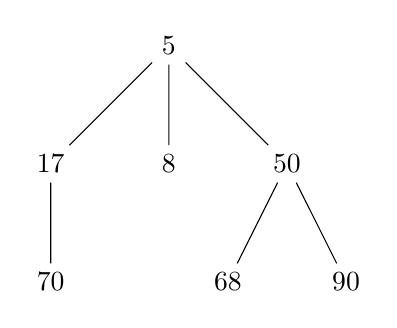
\begin{tikzpicture}
      \node {5}
        child {node {17}
          child {node {70}}}
        child {node {8}}
        child {node {50}
          child {node {68}}
          child {node {90}}};
    \end{tikzpicture}
    \caption{Un ejemplo de \emph{pairing heap}}
    \label{fig:pairing-heap}
  \end{figure}
  Por ahora supondremos esta representación abstracta,
  más adelante discutiremos una estructura concreta.

  Obtener el mínimo
  (\(\mathrm{find\_min}(H)\))
  es acceder a la raíz,
  la operación \(\mathrm{meld}(H_1, H_2)\)
  es poner el árbol con raíz mayor debajo de la raíz del otro
  (elegidos arbitrariamente en caso de empate).
  La operación \(\mathrm{insert}(H, x)\)
  es crear un nuevo árbol con \(x\) de raíz,
  y luego unirlo con el existente.
  Todas tienen costo constante.

  Efectuar \(\mathrm{decrease\_key}(H, x, \Delta)\)
  podría hacerse ajustando la clave de \(x\)
  siempre que no resulte menor que la de su padre,
  o tomando el \emph{\foreignlanguage{english}{heap}} con \(x\) de raíz,
  eliminando \(x\) de él
  (esencialmente la operación \(\mathrm{delete\_min}(H)\)
   en ese subárbol)
  y uniéndolo con el resto.
  Luego insertamos el objeto \(x\) modificado.
  Por simplicidad,
  usaremos siempre la segunda opción
  (acceder al padre es costoso en la estructura que plantearemos más adelante).

  La operación central,
  \(\mathrm{delete\_min}(H)\) es más delicada.
  Al eliminar la raíz,
  quedan varios árboles huérfanos,
  que deben unirse.
  En el peor caso,
  todos los demás objetos son raíces,
  con lo que el costo de hacer esto en forma natural es \(O(n)\).
  La propuesta más simple,
  que llaman \emph{\foreignlanguage{english}{two pass pairing heaps}},
  es como sigue:
  al eliminar la raíz,
  quedan cero o más árboles.
  Estos los unimos a pares,
  partiendo desde el más nuevo
  (suponemos que se agregan árboles a la izquierda),
  y los pares se acumulan luego del más viejo al más nuevo
  (de derecha a izquierda,
   en nuestro orden).
  La figura~\ref{fig:ph-delete-min} muestra la operación.
  Debe considerarse que los nodos hijos a su vez son raíces de árboles,
  que se mantienen intactos.
  Note que el efecto es crear árboles con menos hijos,
  en el ejemplo la primera operación \(\mathrm{delete\_min}\) es cara,
  pero las siguientes serán baratas.
  \begin{figure}[ht]
    \centering
    \subfloat[Original]{
      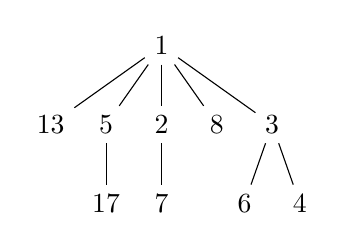
\begin{tikzpicture}[sibling distance = 2em, level distance = 1cm]
        \node {1}
          child {node {13}}
          child {node {5}
            child {node{17}}}
          child {node {2}
            child {node {7}}}
          child {node {8}}
          child {node {3}
            child {node {6}}
            child {node {4}}};
      \end{tikzpicture}
      \label{subfig:ph-dm-original}
    }
    \hspace*{3.75em}
    \subfloat[Parear]{
      \begin{tikzpicture}[sibling distance = 2em, level distance = 1cm]
        \node (r1) {13};
        \node [right = of r1] (r2) {2}
          child {node {5}
            child {node {17}}}
          child {node {7}};
        \node [right = of r2] (r3) {3}
          child {node {8}}
          child {node {6}}
          child {node {4}};
      \end{tikzpicture}
      \label{subfig:ph-dm-parear}
    }
    \hspace*{3.75em}
    \subfloat[Acumular]{
      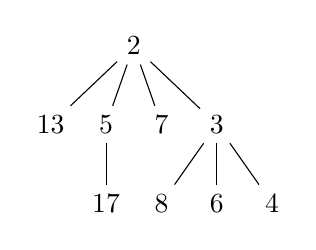
\begin{tikzpicture}[sibling distance = 2em, level distance = 1cm]
        \node {2}
          child {node {13}}
          child {node {5}
            child {node {17}}}
          child {node {7}}
          child {node {3}
            child {node {8}}
            child {node {6}}
            child {node {4}}};
      \end{tikzpicture}
      \label{subfig:ph-dm-acumular}
    }
    \caption{Operación \(\mathrm{delete\_min}\)}
    \label{fig:ph-delete-min}
  \end{figure}

\subsection{Estructura concreta}
\label{sec:ph-concreta}

  Dadas las operaciones que estamos efectuando con los árboles,
  es natural la representación enlazada mediante punteros al primer hijo
  y una lista doblemente enlazada de los hijos,
  con los punteros extremos de la lista apuntando al padre,
  junto con indicación si el nodo es primero o último en la lista.
  Esto permite agregar o eliminar elementos en tiempo \(O(1)\),
  y tener acceso al padre por ejemplo en caso que se quede sin hijos.
  En esta representación todas las operaciones toman tiempo \(O(1)\),
  salvo \(\operatorname{delete\_min}\),
  \(\operatorname{delete}\) y \(\operatorname{decrease\_key}\).

\subsection{Análisis amortizado}
\label{sec:ph-analisis-amortizado}

  Definimos el \emph{tamaño} de \(x\) en un un árbol,
  anotado \(s(x)\),
  como el número de nodos en el subárbol con \(x\) de raíz
  (incluyendo a \(x\));
  y su \emph{rango} como \(r(x) = \log_2 s(x)\).
  Usamos el método potencial,
  con función potencial de un conjunto de árboles:
  \begin{equation}
    \label{eq:ph-phi}
    \Phi(H)
      = \sum_{x \in H} r(x)
  \end{equation}
  El potencial de un conjunto vacío de árboles es \num{0},
  y el potencial nunca es negativo.

  Observamos que el rango de un nodo en un árbol de \(n\) nodos
  está entre \num{0} y \(\log_2 n\).
  Las operaciones \(\mathrm{make\_heap}\)
  y \(\mathrm{find\_min}\) no afectan a \(\Phi\),
  ya que no cambian el rango de ningún nodo;
  su costo amortizado es \(O(1)\).
  Si el número total de nodos es \(n\),
  las operaciones \(\operatorname{insert}\),
  \(\operatorname{meld}\) y \(\operatorname{decrease\_key}\)
  tienen costo amortizado \(O(\log n)\),
  cada una de ellas causa un aumento de potencial acotado por \(\log_2 n + 1\).
  Esto porque la raíz menor aumenta de rango,
  y en menos de \(\log_2 n\)
  (adquiere cuando más \(n - 1\) nuevos descendientes);
  y en caso de \(\mathrm{insert}\) estamos agregando un nuevo nodo,
  que aporta \num{1}.

  La operación \(\mathrm{delete\_min}(H)\) es más difícil de analizar.
  Sea \(H\) un \emph{\foreignlanguage{english}{heap}} de \(n\) nodos
  de raíz \(x\),
  y llamemos \(x_i\) el \(i\)\nobreakdash-ésimo hijo de \(x\).
  Buscamos acotar el número de operaciones
  al reconstruir un \emph{\foreignlanguage{english}{heap}}
  de los árboles con raíces \(x_1, \dotsc, x_k\).
  El tiempo de ejecución de esta operación es uno más
  de los enlaces de nodos efectuados.
  Los enlaces en el primer paso
  (parear)
  son al menos tantos como en el segundo paso
  (acumular).
  Cargaremos \num{2} por enlace en el primer paso.

\section*{Ejercicios}
\label{sec:ejercicios-26-seq2}

  \begin{enumerate}
  \item
    Escriba las operaciones de \emph{\foreignlanguage{english}{pairing heap}}
    como una clase por ejemplo en \cplusplus{} o Java.
  \end{enumerate}

\bibliography{../referencias}

%%% Local Variables:
%%% mode: latex
%%% TeX-master: "../INF-221_notas"
%%% ispell-local-dictionary: "spanish"
%%% End:

% LocalWords:  autoorganizantes english Move To Front MTF Splay trees
% LocalWords:  desbalanceado AVL portable splay Pairing Heaps heap
% LocalWords:  pairing heaps rank ruma computines two pass ésimo
